\part{Modelo Escala}

\section{Resultados}

\subsection{Calculo Permeabilidad Muestra}

\subsection{Aplicacion Diferencias Finitas}

Se determina un caudal de 0.008972885614821659 m/s

\subsection{Licuefaccion}

A continuacion se presenta un video (ver en Adobe Acrobat) de la falla observada por licuefaccion en la maqueta a escala.

\begin{center}
    \includemedia[
        width=0.5625\textwidth, % Relación de aspecto 9:16 (altura mayor que el ancho)
        height=\textwidth,
        activate=onclick,
        addresource=VIDEOS/licuefaccion.mp4,
        flashvars={
            source=VIDEOS/licuefaccion.mp4
        }
    ]{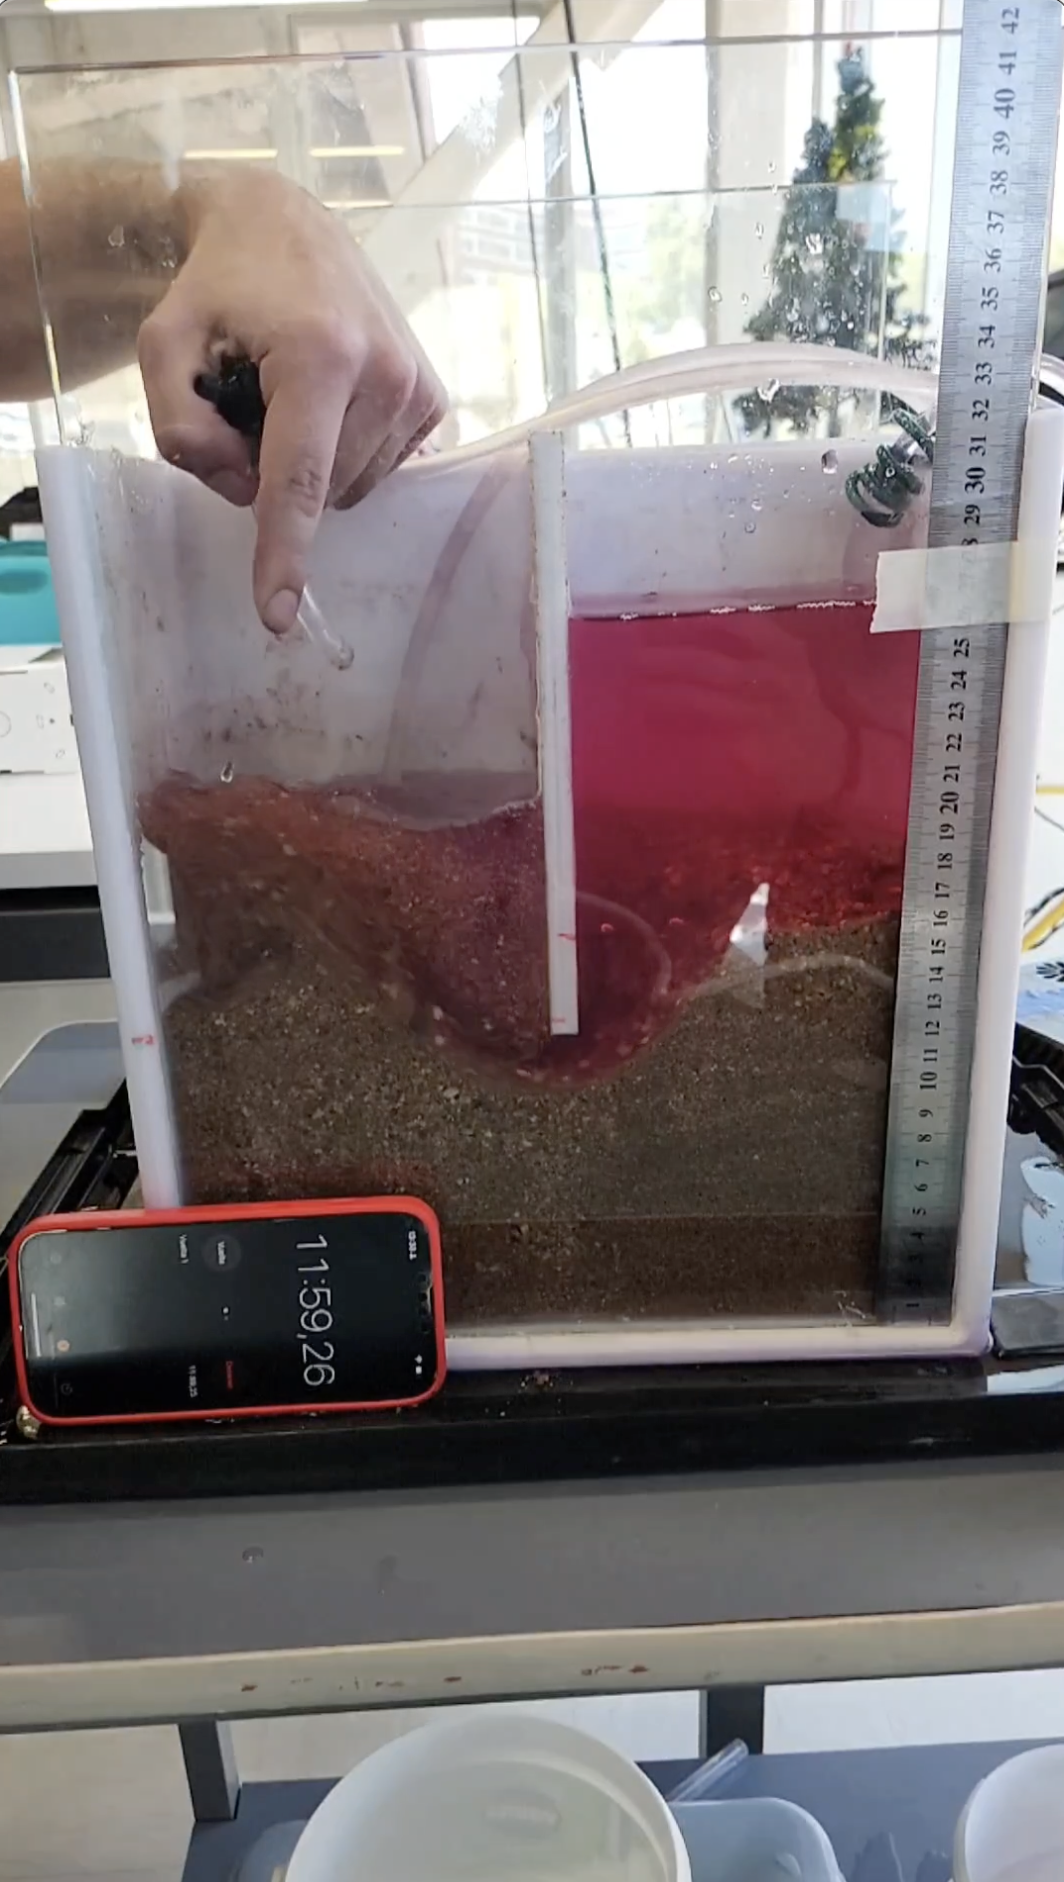
\includegraphics[width=\textwidth]{VIDEOS/miniatura_licuefaccion.png}}{VPlayer.swf}
\end{center}

Las medidas registradas son las siguientes:

\begin{table}[H]
    \centering
    \begin{tabular}{|c|c|c|c|c|c|c|c|}
    \hline
    Caso & $a_1$ & $b_1$ & $c_1$ & $a_2$ & $b_2$ & $c_2$ & $d$ \\ \hline
    Licuefaccion    & 0.0   & 14.5   & 15.5  & 15  & 2.5   & 12.5  & 0.5 \\ \hline
    \end{tabular}
    \caption{Medidas para la Licuefaccion [cm]}
    \label{tab:medidas1}
\end{table}
    

Posteriormente se realizo un mapa de calor correspondiente a la presion de poros en la licuefaccion:

\begin{figure}[H]
    \centering
    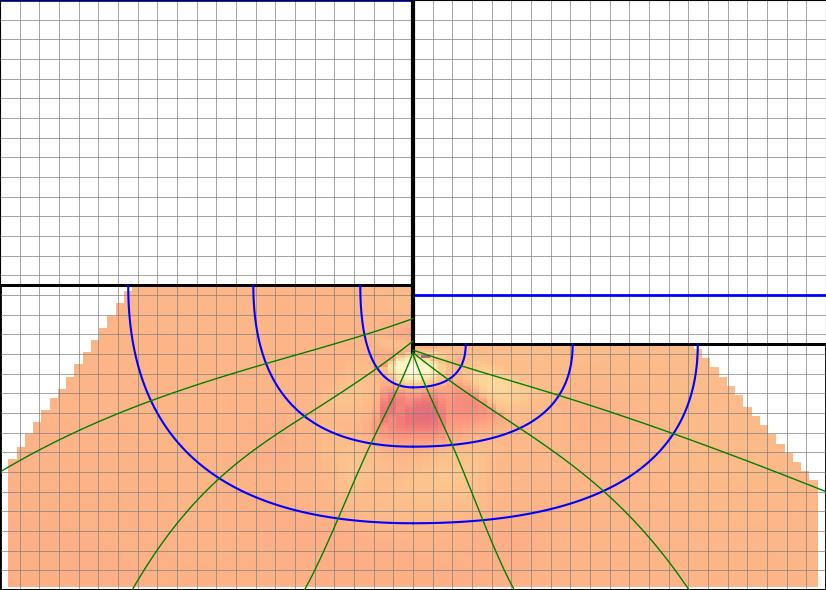
\includegraphics[width=0.5\textwidth]{GRAFICOS/caso_licuefaccion_presion_poros.jpg}
    \caption{Mapa de Calor Licuefaccion}
    \label{fig:maqueta_licuefaccion}
\end{figure}

Es interesante notar como se produce un gran aumento de presion bajo la ataguia, lo cual se observa en el video, ya que ese es el punto esperado de falla.
\\ \\
Ademas, se calculo el mismo caso segun diferencias finitas:

\begin{figure}[H]
    \centering
    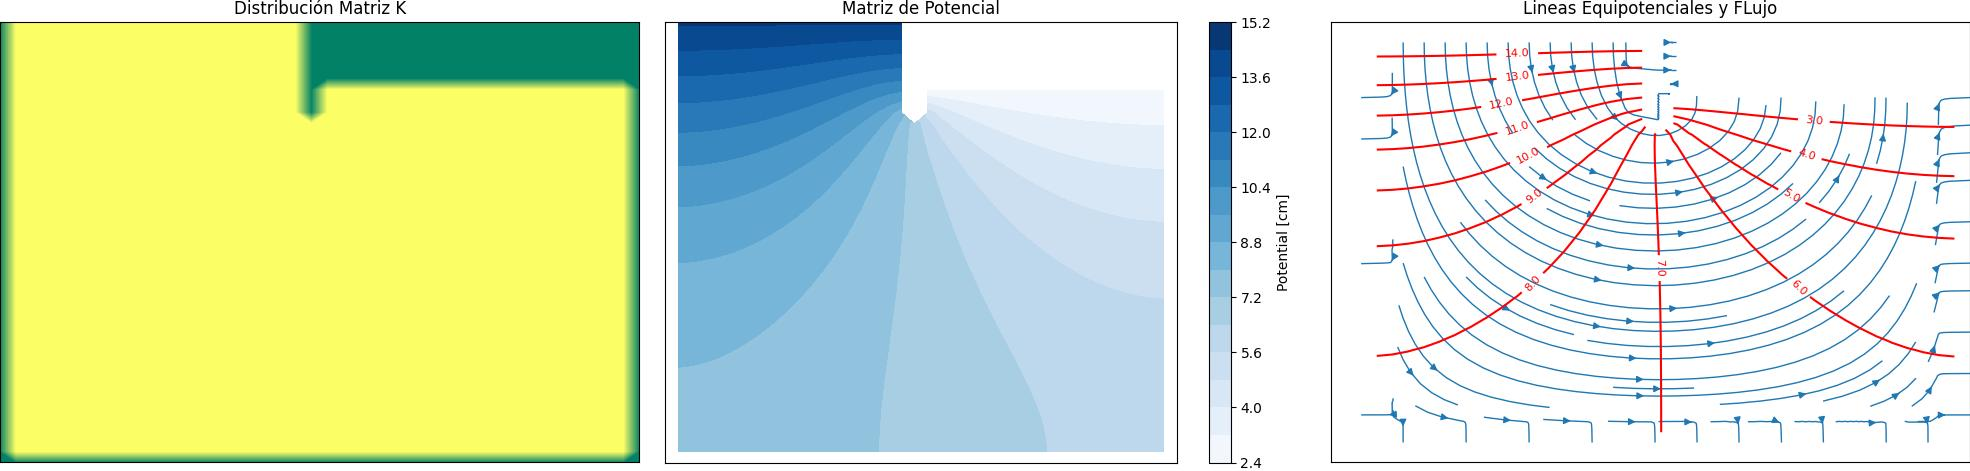
\includegraphics[width=1\textwidth]{GRAFICOS/laplace_caso_licuefaccion_escala_cm.jpg}
    \caption{Laplace Caso Licuefaccion}
    \label{fig:maqueta_licuefaccion_diferencias_finitas}
\end{figure}